\chapter{SOLID}
SOLID ist ein Akronym für fünf fundamentale Prinzipien der objektorientierten Programmierung:
\begin{enumerate}
    \item Single Responsibility Principle (SRP)
    \item Open Closed Principle (OCP)
    \item Liskov Substitution Principle (LSP)
    \item Interface Segregation Principle (ISP)
    \item Dependency Inversion Principle (DIP)
\end{enumerate}
Sie sollen dazu beitragen, dass Software-Systeme leichter zu verstehen, zu entwickeln, zu testen und zu warten sind. \cite{martin.2017}
\section{Analyse Single-Responsibility-Principle (SRP)}
% jeweils eine Klasse als positives und negatives Beispiel für SRP;  jeweils UML der Klasse und Beschreibung der Aufgabe bzw. der Aufgaben und möglicher Lösungsweg des Negativ-Beispiels (inkl. UML)
Das Prinzip besagt, dass eine Klasse nur eine einzige Verantwortung und Aufgabe haben sollte. Durch die Aufteilung von Aufgaben an mehrere Klassen wird die Klasse lesbarer, wartbarer und hat nur einen Grund geändert zu werden. \cite{martin.2017}
\newpage
\subsection{Positiv-Beispiel}
Ein Beispiel einer Klasse, welche dieses Prinzip umsetzt, ist die Klasse UserBuild aus der Adapter Schicht, wie in Abbildung \ref{fig:UMLUserBuild} zu sehen.
\begin{figure}[ht]
    \centering
    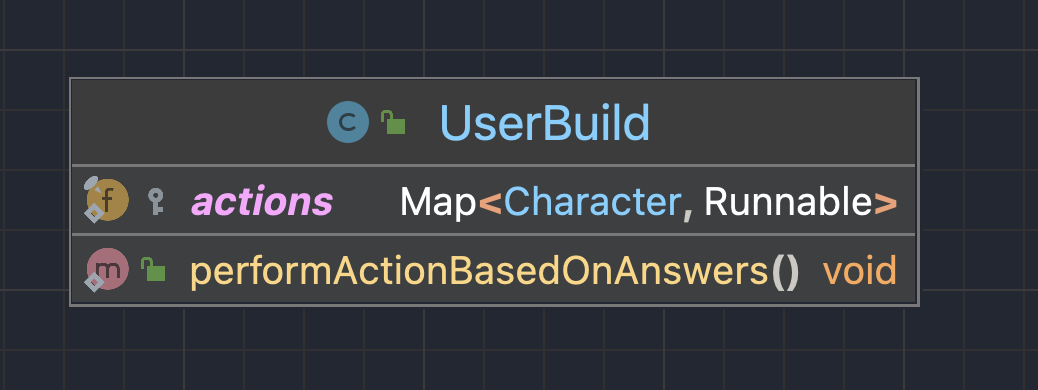
\includegraphics[width=0.4\textwidth]{Bilder/UB.png}
    \caption{Positiv Beispiel SRP der Klasse (UserBuild)}
    \label{fig:UMLUserBuild}
\end{figure}
Ihre primäre Aufgabe ist es, basierend auf der Summe der Character aus den Fragen, die passende Simpsons Figur zu erstellen. 
\subsection{Negativ-Beispiel}
Die Klasse GameTerminal aus der Adapter Schicht hat, wie in Abbildung \ref{fig:UMLGameTerminal} zu sehen, mehrere Aufgaben. Sie ist neben der Erstellung eines Banners und Textes zur Begrüßung des Spieler zusätzlich für die Ausgabe der Fragen und Resultate zuständig.
\begin{figure}[ht]
    \centering
    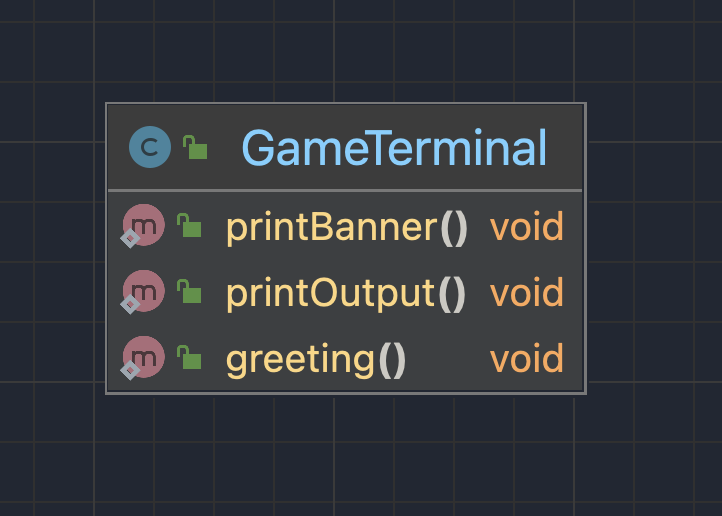
\includegraphics[width=0.3\textwidth]{Bilder/GT.png}
    \caption{Negativ Beispiel SRP der Klasse (GameTerminal)}
    \label{fig:UMLGameTerminal}
\end{figure}
Diese Aufgaben sollten in zwei verschiedene Klassen aufgeteilt werden, um die Lesbarkeit und Wartbarkeit zu verbessern.
\newpage
\section{Analyse Open-Closed-Principle (OCP)}
% jeweils eine Klasse als positives und negatives Beispiel für OCP;  jeweils UML der Klasse und Analyse mit Begründung, warum das OCP erfüllt/nicht erfüllt wurde – falls erfüllt: warum hier sinnvoll/welches Problem gab es? Falls nicht erfüllt: wie könnte man es lösen (inkl. UML)?
Ein Prinzip, welches besagt, dass Klassen offen für Erweiterungen, aber geschlossen für Änderungen sein sollten. Das bedeutet, dass Änderungen an einer Klasse vermieden werden, sobald sich die Bedingungen ändern. \cite{martin.2017}
\subsection{Positiv-Beispiel}
Im Quiz finden sich 10 Figuren aus dem Simpsons Universum, welche alle aus der Klasse SimpsonsCharacter, wie in Abbildung \ref{fig:UMLSimpsonsCharacter} zu sehen, hervorgehen.

\begin{figure}[ht]
    \centering
    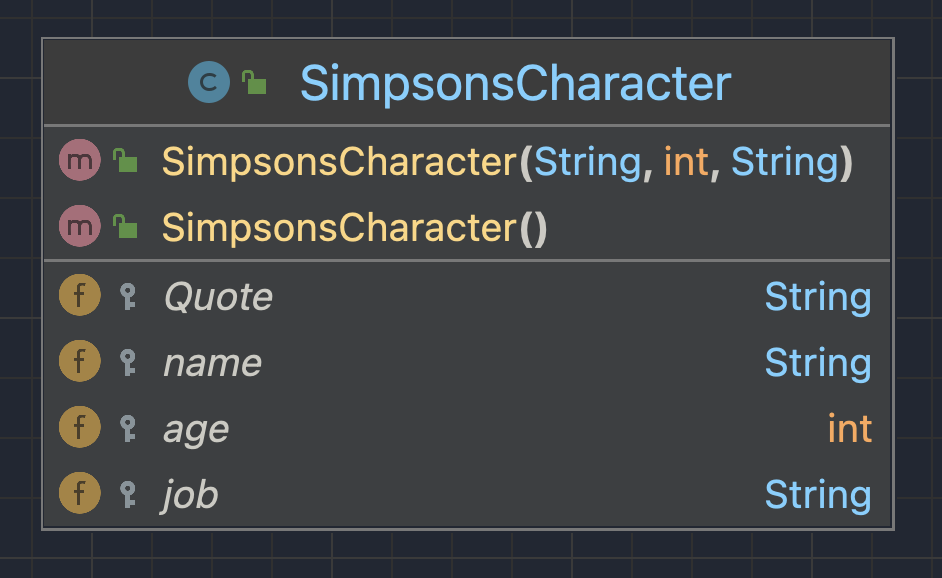
\includegraphics[width=0.3\textwidth]{Bilder/SC.png}
    \caption{Positiv Beispiel OCP der Klasse (SimpsonsCharacter)}
    \label{fig:UMLSimpsonsCharacter}
\end{figure}
Egal wie viele Figuren durch beispielsweise eine Erweiterung noch hinzugefügt werden, die Klasse SimpsonsCharacter muss nicht verändert werden, da sie nur die Grundfunktionen der Figuren enthält.
\subsection{Negativ-Beispiel}
Sollte durch eine Erweiterung eine neuer Figur implementiert werden, wäre die Klasse UserBuild aus Abbildung \ref{fig:UMLUserBuild} ein Verstoss gegen das OCP, da sie bei jeder neuen Figur angepasst werden müsste. Dies ließe sich durch die Auslagerung der Figuren in ein Interface lösen, welches dann als Erweiterung in die Klasse implementiert werden kann.
\section{Analyse Interface-Segreggation- (ISP)}
% jeweils eine Klasse als positives und negatives Beispiel für entweder LSP oder ISP oder DIP);  jeweils UML der Klasse und Begründung, warum man hier das Prinzip erfüllt/nicht erfüllt wird
Das Prinzip besagt, dass eine Klasse nicht von Methoden abhängig sein sollte, die sie nicht benötigt. Durch die Aufteilung von Schnittstellen in kleinere, spezifischere Schnittstellen können unnötige Abhängigkeiten vermieden werden.
\subsection{Positiv-Beispiel}
Ein Beispiel, welche das Prinzip erfüllt, ist das Interface CharacterAction, wie in Abbildung \ref{fig:UMLCharacterAction} zu sehen. Es enthält nur die Methoden, welche für die Figuren benötigt werden. Information über beispielsweise die Features eines Arbeitsplatzes der Figur sind in ein separates Interface ausgelagert worden.
\begin{figure}[ht]
    \centering
    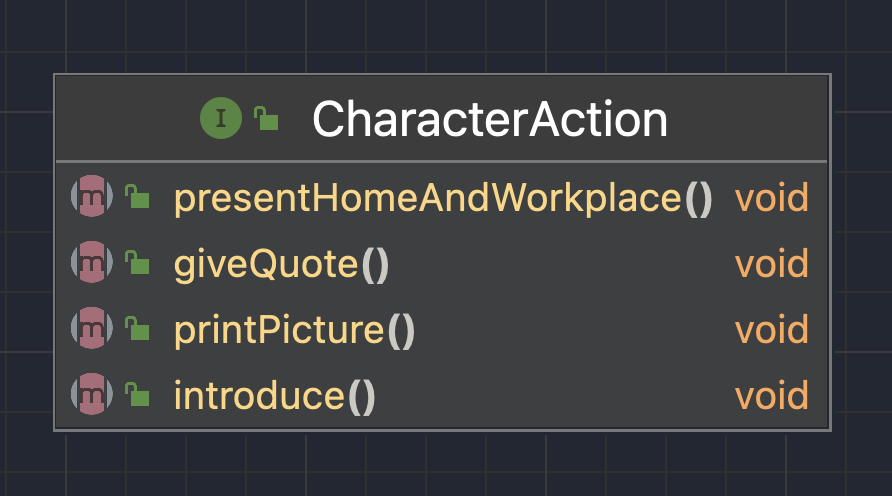
\includegraphics[width=0.3\textwidth]{Bilder/CI.png}
    \caption{Positiv Beispiel ISP der Klasse (CharacterAction)}
    \label{fig:UMLCharacterAction}
\end{figure}

\subsection{Negativ-Beispiel}
Um das genannte Beispiel ins Negative zu kehren, wäre lediglich ein Erweitern des Interfaces um die Methoden aus dem Interface WorkplaceFeatures, wie in Abbildung \ref{fig:UMLWorkplaceFeatures} zu sehen, möglich. Dies würde als Konsequenz bedeuten, dass die Klasse SimpsonsCharacter zusätzlich die Methoden für die Arbeitsplätze verarbeiten müsste und somit unnötige Abhängigkeiten entstehen würden.
\begin{figure}[ht]
    \centering
    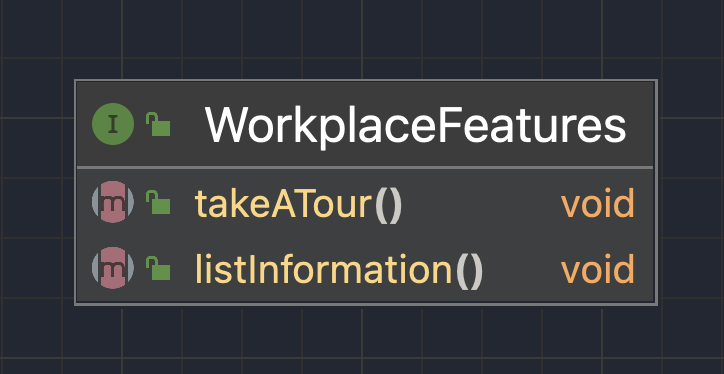
\includegraphics[width=0.3\textwidth]{Bilder/WF.png}
    \caption{Negativ Beispiel ISP der Klasse (WorkplaceFeatures)}
    \label{fig:UMLWorkplaceFeatures}
\end{figure}